%%%                         Louis-Thibault GAUTHIER                       %%%




\newpage


\section{Espaces vectoriels}


\subsection{$1^{ \mbox{\tiny ères}}$  propriétés}


\Def{ \label{ev}
	Soit $E$ un ensemble non vide, que l'on appelera l'ensemble des  \textcolor{gold2}{vecteurs}. Soit $\KK$ un corps, $\KK = \RR$ systématiquement en ECG, et quasi-systématiquement $\RR$ ou $\CC$ dans les autres filières.\\
	Un \textcolor{gold2}{espace vectoriel sur $\KK$},  est un triplet \textcolor{gold2}{$(E,+_E,\cdot_{\KK,E})$}, muni de lois $+_E$, et $\cdot_{\KK,E}$, c'est à dire d'applications :
	\[
		+_E 
		\left\{ 
			\begin{array}{ccc}
				E  \times E &\to & E \\
				\left( x, y \right) & \mapsto & x+_E y
			\end{array}
		\right.
		\qquad
		\cdot_{\KK,E} 
		\left\{ 
			\begin{array}{ccc}
				\KK \times E &\to &E \\
				\left( \lambda,x \right) & \mapsto & \lambda \cdot_{\KK,E} x
			\end{array}
		\right.
	\]
	Que l'on note le plus généralement $+$ et $\cdot$ lorsqu'il n'y a pas de risque de confusion, et tels que, si on se place sur $\KK:= \RR$ :
	\begin{enumerate}
		\item $\forall (u,v)\in E^2; u +v = v+u$. Commutativité.
		\item $\forall (u,v,w)\in E^3; (u+v) + w = u + (v+w)$.  Associativité. On note alors plus simplement $u+v+w$.
		\item $\exists 0_E \in E, \forall u \in E;  u+0_E = u  =0_E +u$. Existence d'un élément neutre.
		\item $\forall u \in E, \exists (-u \in E); u+ (-u) = 0_E = (-u) + u$. Existence d'un inverse.
		\item $\forall u \in E ; 1 \cdot u= u$.
		\item $\forall \lambda \in \RR, \forall (u,v) \in E; \lambda \cdot (u + v) = \lambda \cdot u +  \lambda \cdot v$. Distributivité.
		\item $\forall (\lambda, \mu) \in \RR^2, \forall u \in E; (\lambda + \mu) \cdot u = \lambda \cdot u + \mu \cdot u$. Distributivité.
		\item $\forall (\lambda,\mu) \in \RR^2, \forall u \in E;  \lambda \cdot (\mu \cdot u) = (\lambda \mu)\cdot u$.
	\end{enumerate}
}


Dans tout ce cours $\textcolor{gold2}{(E,+,\cdot)}$ désigne un espace vectoriel sur $\KK$ ($\RR$ pour les ECG), que l'on notera parfois plus succintement $\textcolor{gold2}{E}$, lorsqu'il n'y pas d'ambiguité sur les lois $+$ et $\cdot$. De même $\textcolor{gold2}{(F,+,\cdot)}$ désigne un autre espace vectoriel sur $\KK$ ($\RR$ pour les ECG toujours)
	
\Rem{
	Précisons que la définition d'un espace vectoriel n'est pas très utile \textbf{en pratique} mais donnons un critière intéressant pour les concours qui permet de déterminer si un ensemble possède une structure d'espace vectoriel (selon les lois usuelles) :
}
		
\Def
{ 
	\label{1908171115}
	Un sous-ensemble $F$ de $E$, est un \textcolor{gold2}{sous-espace vectoriel}  de $(E,+,\cdot)$, si il vérifie les conditions suivantes :
	\begin{enumerate}
		\item $0_E \in F$. C'est à dire \og Le vecteur nul de $E$ appartient à $F$ \fg.
		\item $\forall (x,y) \in F^2; \forall (\lambda, \mu) \in \KK^2, \quad (\lambda \cdot x + \mu \cdot y) \in F$. C'est à dire :  \og $F$ est stable par combinaisons linéaires \fg.
	\end{enumerate}
}

	
\Prop
{
	Pour la stabilité par combinaisons linéaires de $F$ : le point \textcolor{gold2}{2} de la définition précédente, on peut se contenter de : 
	\[ 
		\forall (x,y) \in F^2; \forall \lambda \in \KK, \quad (\lambda \cdot x +  y) \in F
	\]
}
	
\Thm
{
		Un sous-espace vectoriel d'un $\KK$-espace vectoriel, est en particulier un $\KK$-espace vectoriel !
}
	
	\Rem[(Extrêmement importante)]
{
		Il faut bien comprendre, qu'en pratique, à la question, montrer que $(T,+_T, \cdot_T)$ est un espace vectoriel, il faudra déterminer de quel espace vectoriel connu il est un sous-espace vectoriel !
}
	
\begin{exo}
	\begin{enumerate}
		\item Soit 
		\[
			F_1 = \left\{ \begin{pmatrix} x\\y\\z \end{pmatrix} \vert x-2y +z =0 \right\} \quad F_2  = \left\{ \begin{pmatrix} x-y \\2x +3y-z \\4x- 3z \end{pmatrix} \vert (x,y,z) \in \RR^3 \right\} 
		\]
		Montrer que $F_1$ et $F_2$ sont des espaces	vectoriels.
	\end{enumerate}
\end{exo}


\Prop[(Espaces vectoriels de référence)]
{
 \label{evréférence}
	Soit $n,p \in \NN^*, r\in \NN$, et $I$ un intervalle de $\RR$ non réduit à un point. Nous connaissons les espaces vectoriels de référence suivant :
	\begin{equation}\label{11817}
		\begin{array}{cccccc}
			\RR^n & \KK^n  &  \RR[X] & \RR_r[X] & \KK[X] & \KK_r[X] \\
			  \RR^{\NN} & \RR^{\RR} &	 \calC^0(I,\RR) & \calC^n(I,\RR) & \calC^{\infty}(I, \RR) &	\calM_n(\RR)\\
			   \calM_{n,p}(\RR) &\calM_n(\KK) & \calM_{n,p}(\KK)
		\end{array} 
	\end{equation}
}

Nous n'allons pas faire de rappels détaillés sur l'ensemble des fonctions polynômiales, pour les ECG, et l'ensemble des polynômes à une indéterminée, et à coefficients dans un corps $\textcolor{vertfoncé}{\KK}$ pour les filières scientifiques. Qui sont notés :  
\[
 \left\{  \begin{array}{lll} \textcolor{gold2}{\RR[x]}  \mbox{ (ECG)} \\ \textcolor{vertfoncé}{\KK[X]} \mbox{ (Maths sup)}  \end{array} \right.
\]
Cependant :

\Def
{
	Posons $n \in \NN^*$. On désigne par 	$\textcolor{gold2}{\RR_n[x]}$ et $\textcolor{vertfoncé}{\KK_n[X]}$ les ensembles :
	\[ 
		\left\{  
			\begin{array}{lll}
				\textcolor{gold2}{\RR_n[x]}  & := &  \left\{  P \in \textcolor{bleu}{\RR[x]}  \mid \textup{deg } P \leq n \right\}\\ 
				\textcolor{vertfoncé}{\KK_n[X]} & := &  \left\{  P 	\in\textcolor{vertfoncé}{\KK[X]}) \mid \textup{deg } P \leq n \right\}\\ 
			\end{array} 
		\right.  
	\]
}

\Prop
{
	Soit $E$ un espace vectoriel. Soit $F_1,F_2$ deux sous-espaces vectoriels quelconques de $E$. Alors $F_1 \cap F_2$ est un sous-espace vectoriel de $E$.
}

En réalité, on a mieux : Voir la proposition \ref{intev} page \pageref{intev}.

\begin{exo}
	Détailler les lois, dans l'équation (\ref{11817}), avec les hypothèses de la proposition \ref{evréférence}, de $\RR[X], \calC^0(I,\RR)$, et $\calM_n(\RR)$. Ainsi que leurs vecteurs nuls. 
	\end{exo}
	
	Par exemple, pour le premier, en faisant l'abus d'écriture de noter verticalement  $\begin{pmatrix} x_1 \\ \vdots \\x_n \end{pmatrix}$ un vecteur $(x_1,\cdots, x_n) \in \RR^n$ : 
	
	
\begin{proof}
	\begin{itemize}
		\item $(\RR^n,+, \cdot)$. Son élément neutre $0_E$, est le vecteur nul : $$\begin{pmatrix} 0 \\\vdots \\0 \end{pmatrix} \in \RR^n$$
		\item et :
			\[ 			
				+
				\left\{ 
					\begin{array}{ccccccll}
						\RR^n  \times \RR^n &\to &\RR^n \\
						\left( \begin{pmatrix} x_1 \\ \vdots \\x_n \end{pmatrix},
						\begin{pmatrix} y_1 \\ \vdots \\y_n \end{pmatrix}\right) & \mapsto &
						\begin{pmatrix} x_1 +y_1 \\ \vdots \\x_n + y_n \end{pmatrix}
					\end{array}
				\right.
				\qquad \cdot  
				\left\{ 
					\begin{array}{ccccccll}
						\RR \times \RR^n &\to &\RR^n \\
						\left( \lambda, \begin{pmatrix} x_1 \\ \vdots \\x_n \end{pmatrix} \right) 	& \mapsto &
						\begin{pmatrix} \lambda x_1 \\ \vdots \\ \lambda x_n \end{pmatrix}
					\end{array}
				\right.
			\]
	\end{itemize}
\end{proof}		

\begin{exo}
	Montrer que :
	\[
		F = \{ P \in \RR[X] \vert P(1) = 0 \} \qquad 	G = \{ (u_n)_{n\in \NN} \vert \forall n \in \NN u_{n+1}=2u_n \}
	\]
	\noindent sont des $\RR$-espaces vectoriels.
\end{exo}

\begin{exo}
	Est-ce que 
	\begin{equation*}
		H = \{ P \in \RR[X] \vert P(0) = 1 \} \qquad I = \{ (u_n)_{n\in \NN} \vert u_1 = 2 \}
	\end{equation*}
	\noindent sont des $\RR$-espaces vectoriels ?
\end{exo}


\subsection{Comb. linéaires}


\Def
{
	Soit $x,x_1,\cdots, x_n$ des vecteurs de $E$. On dit que $x$ est \textcolor{gold2}{combinaison linéaire} des $x_1, \cdots ,x_n$, lorsqu'il existe $n$ scalaires $\lambda_1,\cdots, \lambda_n \in \RR$, tels que :
	\[ 
		x  = \lambda_1 x_1 +\cdots + \lambda_n x_n = \sum_{i= 1}^n \lambda_i x_i 
	\]
}

\example
	Le vecteur $x:=\begin{pmatrix} 1 \\-2 \end{pmatrix}$ de $\RR^2$, est combinaison linéaire de $x_1 := \begin{pmatrix} 1 \\0 \end{pmatrix}$, et $x_2 := \begin{pmatrix} 0 \\1 \end{pmatrix}$, pour $\lambda_1 :=1$, et $\lambda_2 := -2$ :
	\[
		x=  \begin{pmatrix} 1 \\-2 \end{pmatrix} = 1 \cdot \begin{pmatrix} 1 \\0 \end{pmatrix} -2 \cdot  \begin{pmatrix} 0 \\1 \end{pmatrix} = 1\cdot x_1 -2 \cdot x_2  
	\]

On peut utiliser les systèmes linéaires comme outils pour résoudre des questions concernant les espaces vectoriels, c'est l'objet de l'exercice suivant :

\begin{exo}  %Savoir et faire ECE1
	\vspace{2pt}
	Soit $u = \begin{pmatrix} 7 \\2\\-6\end{pmatrix}, u_1 = \begin{pmatrix} 2\\1\\-1 \end{pmatrix},u_2 = \begin{pmatrix} 1\\1\\1 \end{pmatrix}, u_3 = \begin{pmatrix}0 \\1 \\2 \end{pmatrix}$. Montrer que $u$ est combinaison linéaire de $u_1,u_2,u_3$.
\end{exo}


\subsection{Le \og Vect \fg}

Soit $E$ un espace vectoriel.


\Prop
{ 
	\label{intev}
	Une intersection de sous-espaces vectoriels de $E$ est un sous-espace vectoriel de $E$.
}

\Defprop[(Hors-programme en ECG)]
{
	\label{140817}
	Soit $A \subset E$. \textcolor{gold2}{L'espace vectoriel engendré} par $A$, est le plus petit sous-espace vectoriel de $E$, qui contienne $A$. Il existe, c'est l'intersection de tous les sous-expaces vectoriels de $E$, qui contiennent $A$ :
	\[ 
	\textup{Vect}(A) = \bigcap_{ E' \mbox{ sous ev de } E \mbox{ tel que }  A \subseteq E'} E'
	\]
	C'est aussi \textcolor{gold2}{l'ensemble des combinaisons linéaires} d'éléments de $A$ :
	\[ 
	\textup{Vect}(A) = \left\{ \sum_{i=1}^n \lambda_i x_i \vert n \in \NN^*; \lambda_i \in \RR ; x_i \in A \right\}
	\]
}

\Rem
{ 
	L'ensemble  $\textup{Vect}(A)$   des combinaisons linéaires d'une famille $A$ (non vide la plupart du temps \footnotemark) de vecteurs d'un \textbf{même} espace vectoriel $E$, est toujours un sous-espace vectoriel de $E$ ! \\
	En ECG, on parle surtout du \og Vect \fg d'une famille finie de vecteurs.
}
\footnotetext{Même si $\textup{Vect}(\varnothing)$ a un sens, on ne le mentionne pas souvent, étant donné le peu d'intérêt qu'il représente.}

Ce qui amène à une définition \og plus concrète \fg :

\Defprop[(Plus appropriée en ECG)]
{
	Soit $n\in \NN^*$. Soit $(x_1,x_2, \cdots, x_n)$ une famille de vecteurs de $E$. Alors on a :
	\[ 
		\textup{Vect}(x_1,x_2, \cdots, x_n) = \left\{  \lambda_1 x_1 + \lambda_2 x_2 + \cdots + \lambda_nx_n \mid \lambda_1, \cdots, \lambda_n \in \RR  \right\}
	\]
}


\subsection{Exemples}


\example
	\[ 
		\textup{Vect}\left(  \begin{pmatrix} 1 \\0 \\ 3 \end{pmatrix}, \begin{pmatrix} -2 \\ 0 \\1 \end{pmatrix} \right) = \left\{ \lambda_1 \cdot  \begin{pmatrix} 1 \\0 \\ 3 \end{pmatrix} + 	\lambda_2 \cdot \begin{pmatrix} -2 \\ 0 \\1 \end{pmatrix}  \mid \lambda_1, \lambda_2 \in \RR \right\}
	\]	

\example


Dessinons, dans le plan $\RR^2$, le sous-espace vectoriel : 	$\textup{Vect}\left(  \begin{pmatrix} 1 \\ 1 \end{pmatrix}\right)$.


\begin{center}
	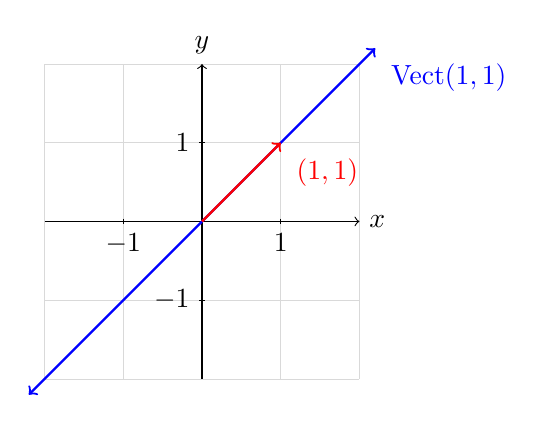
\begin{tikzpicture}[scale=1]
	% Grille de fond
	\draw[very thin,gray!30] (-2,-2) grid (2,2);
	
	% Axes
	\draw[->] (-2,0) -- (2,0) node[right] {$x$};
	\draw[->] (0,-2) -- (0,2) node[above] {$y$};
	
	% Graduations principales
	\foreach \x in {-1,1}
	{
		\draw (\x cm,1pt) -- (\x cm,-1pt) node[anchor=north] {$\x$};
		\draw (1pt,\x cm) -- (-1pt,\x cm) node[anchor=east] {$\x$};
	}
	
	% Droite vectorielle en bleu
	\draw[<->,blue, thick] (-2.2,-2.2) -- (2.2,2.2) node[below right = 2pt] {$\textcolor{blue}{\textup{Vect}(1,1)}$};
	
	% Vecteur (1,1) en rouge avec étiquette plus basse
	\draw[->, red, thick] (0,0) -- (1,1) node[below right=2pt] {$(1,1)$};
\end{tikzpicture}
\end{center}

Pour visualiser $\textup{Vect}\left(  \begin{pmatrix} 1 \\ 1 \end{pmatrix}\right)$, vous devez comprendre que cet ensemble est constitué de tous les multiples scalaires du vecteur $\left(  \begin{pmatrix} 1 \\ 1 \end{pmatrix}\right)$, par exemple il y a $2\cdot \begin{pmatrix} 1 \\ 1 \end{pmatrix}= \begin{pmatrix} 2 \\ 2 \end{pmatrix}$ mais aussi $ \begin{pmatrix} -3.5 \\ -3.5 \end{pmatrix}$ etc.

\example

	On remarque qu'on obtient un plan vectoriel :
	Dessinons, dans l'espace $\RR^3$, le sous espace vectoriel :
	
	\[
		 \textup{Vect}
		 \left(
			 \begin{pmatrix}
				 -1 \\
				 1 \\
				 1 
				\end{pmatrix}
			 \begin{pmatrix}
				 1 \\
				 1 \\
				 1
			 \end{pmatrix}
		 \right)
	\]



\begin{center}

	\tdplotsetmaincoords{60}{70}
	
		\begin{tikzpicture}[scale=3,tdplot_main_coords]
	
	% Axes 3D
	\draw[->] (-1,0,0) -- (2,0,0) node[right] {$x$};
	\draw[->] (0,-0.5,0) -- (0,2,0) node[right] {$y$};
	\draw[->] (0,0,-0.5) -- (0,0,2) node[above] {$z$};
	
	% Graduations principales
	\foreach \x in {1}
	{
		\draw[dotted] (\x,0,0) -- (\x,0,\x);
		\draw[dotted] (\x,0,\x) -- (0,0,\x);
		\draw (\x,0,0) node[below] {$\x$};
		\draw (0,\x,0) node[below] {$\x$};
		\draw (0,0,\x) node[left] {$\x$};
	}
	
	% Plan vectoriel recentré et élargi
	\draw[green!30, fill=green!10, opacity=0.5] 
	(0,-0.2,-0.2) --    % coin inférieur gauche
	(2.2,1.2,1.2) --     % coin supérieur droit
	(1.2,2,2) --         % coin supérieur
	(-1.5,1.0,1.0) --      % coin inférieur
	cycle;
	
	% Extension du plan (lignes de niveau réorganisées)
	\draw[dashed, green!50] (-1.5,0.4,0.4) -- (2.2,0.4,0.4);
	\draw[dashed, green!50] (-1.5,0.8,0.8) -- (2.2,0.8,0.8);
	\draw[dashed, green!50] (-1.5,1.2,1.2) -- (2.2,1.2,1.2);
	\draw[dashed, green!50] (0.2,1.6,1.6) -- (2.0,1.6,1.6);  % Ligne encore plus à droite
	\draw[dashed, green!50] (0.6,2.0,2.0) -- (1.6,2.0,2.0);  % Ligne encore plus à droite
	
	% Les deux vecteurs générateurs
	\draw[->, red, thick] (0,0,0) -- (1,1,1) node[above right] {$\vec{u_1}(1,1,1)$};
	\draw[->, blue, thick] (0,0,0) -- (-1,1,1) node[above left=-6pt] {$\vec{u_2}(-1,1,1)$};
	
	% Étiquette du plan
	\node[above = 8pt] at (0.6,1.7,1.7) {$\textcolor{vertfoncé}{\textup{Vect}(\vec{u_1},\vec{u_2})}$};
\end{tikzpicture}


\end{center}

\begin{figure}[h]
	
	\begin{tikzpicture}[baseline]
		\node[anchor=base,xshift=0cm] (sch1) {
			\tdplotsetmaincoords{60}{-65}
				\begin{tikzpicture}[scale=1.5,tdplot_main_coords]
	
	% Axes 3D
	\draw[->] (-1,0,0) -- (2,0,0) node[right] {$x$};
	\draw[->] (0,-0.5,0) -- (0,2,0) node[right] {$y$};
	\draw[->] (0,0,-0.5) -- (0,0,2) node[above] {$z$};
	
	% Graduations principales
	\foreach \x in {1}
	{
		\draw[dotted] (\x,0,0) -- (\x,0,\x);
		\draw[dotted] (\x,0,\x) -- (0,0,\x);
		\draw (\x,0,0) node[below] {$\x$};
		\draw (0,\x,0) node[below] {$\x$};
		\draw (0,0,\x) node[left] {$\x$};
	}
	
	% Plan vectoriel recentré et élargi
	\draw[green!30, fill=green!10, opacity=0.5] 
	(0,-0.2,-0.2) --    % coin inférieur gauche
	(2.2,1.2,1.2) --     % coin supérieur droit
	(1.2,2,2) --         % coin supérieur
	(-1.5,1.0,1.0) --      % coin inférieur
	cycle;
	
	% Extension du plan (lignes de niveau réorganisées)
	\draw[dashed, green!50] (-1.5,0.4,0.4) -- (2.2,0.4,0.4);
	\draw[dashed, green!50] (-1.5,0.8,0.8) -- (2.2,0.8,0.8);
	\draw[dashed, green!50] (-1.5,1.2,1.2) -- (2.2,1.2,1.2);
	\draw[dashed, green!50] (0.2,1.6,1.6) -- (2.0,1.6,1.6);  % Ligne encore plus à droite
	\draw[dashed, green!50] (0.6,2.0,2.0) -- (1.6,2.0,2.0);  % Ligne encore plus à droite
	
	% Les deux vecteurs générateurs
	\draw[->, red, thick] (0,0,0) -- (1,1,1) node[above right] {\tiny$\vec{u_1}(1,1,1)$};
	\draw[->, blue, thick] (0,0,0) -- (-1,1,1) node[above left=-6pt] {\tiny$\vec{u_2}(-1,1,1)$};
	
	% Étiquette du plan
	\node[above = 5pt] at (0.6,1.7,1.7) {\tiny$\textcolor{vertfoncé}{\textup{Vect}(\vec{u_1},\vec{u_2})}$};
\end{tikzpicture}

		};
		
		\node[anchor=base,yshift=-0.5cm,xshift=4cm] (sch2) {
			\tdplotsetmaincoords{60}{35}
				\begin{tikzpicture}[scale=1.5,tdplot_main_coords]
	
	% Axes 3D
	\draw[->] (-1,0,0) -- (2,0,0) node[right] {$x$};
	\draw[->] (0,-0.5,0) -- (0,2,0) node[right] {$y$};
	\draw[->] (0,0,-0.5) -- (0,0,2) node[above] {$z$};
	
	% Graduations principales
	\foreach \x in {1}
	{
		\draw[dotted] (\x,0,0) -- (\x,0,\x);
		\draw[dotted] (\x,0,\x) -- (0,0,\x);
		\draw (\x,0,0) node[below] {$\x$};
		\draw (0,\x,0) node[below] {$\x$};
		\draw (0,0,\x) node[left] {$\x$};
	}
	
	% Plan vectoriel recentré et élargi
	\draw[green!30, fill=green!10, opacity=0.5] 
	(0,-0.2,-0.2) --    % coin inférieur gauche
	(2.2,1.2,1.2) --     % coin supérieur droit
	(1.2,2,2) --         % coin supérieur
	(-1.5,1.0,1.0) --      % coin inférieur
	cycle;
	
	% Extension du plan (lignes de niveau réorganisées)
	\draw[dashed, green!50] (-1.5,0.4,0.4) -- (2.2,0.4,0.4);
	\draw[dashed, green!50] (-1.5,0.8,0.8) -- (2.2,0.8,0.8);
	\draw[dashed, green!50] (-1.5,1.2,1.2) -- (2.2,1.2,1.2);
	\draw[dashed, green!50] (0.2,1.6,1.6) -- (2.0,1.6,1.6);  % Ligne encore plus à droite
	\draw[dashed, green!50] (0.6,2.0,2.0) -- (1.6,2.0,2.0);  % Ligne encore plus à droite
	
	% Les deux vecteurs générateurs
	\draw[->, red, thick] (0,0,0) -- (1,1,1) node[above right] {\tiny$\vec{u_1}(1,1,1)$};
	\draw[->, blue, thick] (0,0,0) -- (-1,1,1) node[above left=-6pt] {\tiny$\vec{u_2}(-1,1,1)$};
	
	% Étiquette du plan
	\node[above = 5pt] at (0.6,1.7,1.7) {\tiny$\textcolor{vertfoncé}{\textup{Vect}(\vec{u_1},\vec{u_2})}$};
\end{tikzpicture}

		};
		
		\node[anchor=base,yshift=-1cm,xshift=8cm] (sch2) {
			\tdplotsetmaincoords{60}{105}
				\begin{tikzpicture}[scale=1.5,tdplot_main_coords]
	
	% Axes 3D
	\draw[->] (-1,0,0) -- (2,0,0) node[right] {$x$};
	\draw[->] (0,-0.5,0) -- (0,2,0) node[right] {$y$};
	\draw[->] (0,0,-0.5) -- (0,0,2) node[above] {$z$};
	
	% Graduations principales
	\foreach \x in {1}
	{
		\draw[dotted] (\x,0,0) -- (\x,0,\x);
		\draw[dotted] (\x,0,\x) -- (0,0,\x);
		\draw (\x,0,0) node[below] {$\x$};
		\draw (0,\x,0) node[below] {$\x$};
		\draw (0,0,\x) node[left] {$\x$};
	}
	
	% Plan vectoriel recentré et élargi
	\draw[green!30, fill=green!10, opacity=0.5] 
	(0,-0.2,-0.2) --    % coin inférieur gauche
	(2.2,1.2,1.2) --     % coin supérieur droit
	(1.2,2,2) --         % coin supérieur
	(-1.5,1.0,1.0) --      % coin inférieur
	cycle;
	
	% Extension du plan (lignes de niveau réorganisées)
	\draw[dashed, green!50] (-1.5,0.4,0.4) -- (2.2,0.4,0.4);
	\draw[dashed, green!50] (-1.5,0.8,0.8) -- (2.2,0.8,0.8);
	\draw[dashed, green!50] (-1.5,1.2,1.2) -- (2.2,1.2,1.2);
	\draw[dashed, green!50] (0.2,1.6,1.6) -- (2.0,1.6,1.6);  % Ligne encore plus à droite
	\draw[dashed, green!50] (0.6,2.0,2.0) -- (1.6,2.0,2.0);  % Ligne encore plus à droite
	
	% Les deux vecteurs générateurs
	\draw[->, red, thick] (0,0,0) -- (1,1,1) node[above right] {\tiny$\vec{u_1}(1,1,1)$};
	\draw[->, blue, thick] (0,0,0) -- (-1,1,1) node[above left=-6pt] {\tiny$\vec{u_2}(-1,1,1)$};
	
	% Étiquette du plan
	\node[above = 5pt] at (0.6,1.7,1.7) {\tiny$\textcolor{vertfoncé}{\textup{Vect}(\vec{u_1},\vec{u_2})}$};
\end{tikzpicture}

		};
	\end{tikzpicture}
	%	\caption{Schémas côte à côte}
	
\end{figure}


Détaillons dans l'exercice suivant une méthode pour écrire un sous-espace vectoriel sous forme de \og $\textup{vect}$ \fg.
	
	
\begin{exo} 
	Soit 
	\[
		F := \left\{ \begin{pmatrix} x-y \\ 2x+3y-z \\4x-3z \end{pmatrix} \mid (x,y,z) \in \RR^3 	\right\}
	\]
	Trouver trois vecteurs $X_1,X_2,X_3$, chacun dans $\RR^3$, tels que $F = \textup{vect}(X_1,X_2,X_3)$.
\end{exo}
	
\Rem{ 
		On a donc montré dans l'exercice précédent, en particulier, que $F$ est sous-espace vectoriel de $\RR^3$. Ceci peut être une méthode pour montrer qu'un ensemble est un espace vectoriel, ou un sous-espace vectoriel. 
}


\noindent	Donnons un exemple légèrement plus subtil :
	
\begin{exo} 
	Soit
	\[
		F := \left\{ \begin{pmatrix}x  \\y \\z \end{pmatrix} \mid x-2y+z=0 \right\}
	\]
	Exprimer $F$ sous forme de \og vect \fg :
\end{exo}



%%%                         Louis-Thibault GAUTHIER                       %%%